\documentclass[12pt,a4paper]{article}
\usepackage[UTF8]{ctex}
\usepackage[backend=biber]{biblatex}
\usepackage{amsmath,amsthm,amssymb,graphicx,multirow,float,caption}
\usepackage{geometry}
\geometry{left=2.54cm, right=2.54cm, top=3.18cm, bottom=3.18cm}
\usepackage{enumitem}
\usepackage{subcaption,booktabs,diagbox}
\setenumerate[1]{itemsep=0pt,partopsep=0pt,parsep=\parskip,topsep=5pt}
\setitemize[1]{itemsep=0pt,partopsep=0pt,parsep=\parskip,topsep=5pt}
\setdescription{itemsep=0pt,partopsep=0pt,parsep=\parskip,topsep=5pt}
\usepackage{adjustbox}
\usepackage[graphicx]{realboxes}
\usepackage{rotating}

\usepackage{titlesec}

\newcommand{\be}[1]{
    \begin{equation}
        #1
    \end{equation}
}

\newcommand{\bfig}[3]{
    \begin{figure}[H]
        \centering
        \includegraphics[width=#1\textwidth]{#2}
        \caption{#3}
    \end{figure}
}

\titleformat{\section}%设置section的样式
{\raggedright\large\bfseries}%右对齐,4号字,加粗
{\thesection .\quad}%标号后面有个点
{0pt}%sep label和title之间的水平距离
{}%标题前没有内容

\title{\vspace{-4cm}\Large 锁相放大器}  %文章标题
\author{\kaishu 学号:202111030007 \hspace{1.5cm} 姓名:郑晓旸 \hspace{1.5cm} 指导老师: 何琛娟}   %作者的名称
\date{}

\begin{document}
\maketitle

\begin{abstract}
    本实验使用锁相放大器研究了参考信号通道特性,得到参考信号与信号源频率相等,幅度为固定值,与信号源无关;研究了相敏检波器 PSD 输出波形和电压与信号源和参考信号的关系,得出其在实验误差允许范围内满足公式(4);
    研究了相关器对谐波的响应情况,得出当输入信号为参考信号的次谐波时,直流输出信号的幅度最大值与倍数成反比;
    研究了干扰信号对PSD直流输出电压的影响,输出电压对干扰信号奇次谐波的抗干扰能力较差。
    研究了相关器对噪声的抑制情况,信噪比改善受到输入端信号、输入噪声以及时间常数影响。
\end{abstract}

\section{引言}

锁相放大器是检测淹没在噪声中微弱信号的常用仪器。它利用待测信号和参考信号的互相关检测原理,实现对信号的窄带化处理,能够有效地抑制噪声,从而实现对信号的检测和跟踪。这种技术在现代科学和工程中有着广泛的应用。

锁相放大器的工作原理基于相干检测,通过将待测信号与参考信号进行相位比较,提取出信号的相干成分。待测信号和参考信号通常具有相同的频率,但可能在相位上有一定差异。通过锁相放大器的混频和滤波处理,可以有效地将噪声与信号分离,使得即使在非常低的信噪比情况下,仍能准确地检测到信号。

锁相放大器广泛应用于物理、化学、生物、电讯、医学等领域。例如,在物理实验中,锁相放大器可以用于检测微弱的光电流信号;在化学实验中,它可以用于测量化学反应过程中产生的微小电信号;在生物实验中,锁相放大器能够检测生物样品中的微弱生物电信号;在电讯领域,它被用于高灵敏度的信号接收和处理;在医学领域,锁相放大器则应用于精确测量心电图和脑电图等生物医学信号。

掌握锁相放大器的工作原理和使用方法,对于科学研究和工程应用具有重要意义。本实验将通过测量锁相放大器的工作参数和特性,详细探讨其工作机制,帮助我们理解如何在实际应用中有效地使用锁相放大器,从而提高信号检测的精度和可靠性。

\section{原理}
\subsection{相关接收}
微弱信号检测的基础是被测信号在时间上具有前后相关性的特点,即两个函数间有一定的关系。相关函数则是表征线性相关的度量。设信号 $f_1(t)$ 为被测信号 $V_s(t)$ 和噪声 $V_n(t)$ 的叠加,$f_2(t)$ 为与被测信号同步的参考信号 $V_r(t)$,则相关函数定义为:

\begin{equation}
R_{12}(\tau) = \lim_{T\rightarrow \infty}\frac{1}{2T}\int_{-\infty}^{\infty} f_1(t) f_2(t + \tau) \, dt
\end{equation}

其中,$f_1(t) = V_s(t) + V_n(t)$。将其代入相关函数的表达式,可以得到:

\begin{equation}
R_{12}(\tau) = \lim_{T\rightarrow \infty}\frac{1}{2T}\int_{-\infty}^{\infty} [V_s(t) + V_n(t)] V_r(t + \tau) \, dt
\end{equation}

可以将上述式子展开为两部分:

\begin{equation}
R_{12}(\tau) = \lim_{T\rightarrow \infty}\frac{1}{2T}(\int_{-\infty}^{\infty} V_s(t) V_r(t + \tau) \, dt + \int_{-\infty}^{\infty} V_n(t) V_r(t + \tau) \, dt)\\
=R_{s r}(\tau)+R_{n r}(\tau)
\end{equation}

分别表示信号与参考信号的相关性和噪声与参考信号的相关性。由于噪声和参考信号不相关,所以 $R_{nr}(\tau) = 0$,故 $R_{12}(\tau) = R_{sr}(\tau)$。因此,利用参考信号与有用信号的相关性,而参考信号与噪声互不相关的性质,通过互相关运算可以有效地削弱噪声的影响,从而把深埋在噪声中的微弱信号检测出来。

锁相放大器的工作原理正是基于上述相关检测的思想。通过对输入信号和参考信号进行相位比较,并利用低通滤波器滤除高频噪声成分,可以显著提高信号的信噪比,使得微弱信号的检测成为可能。具体来说,锁相放大器首先将输入信号与参考信号混频,得到包含信号频率成分的输出信号。然后,经过低通滤波,仅保留信号的低频成分,从而实现对微弱信号的提取。

\subsection{相干检测的实现}

相干检测器是实现求参考信号和被测信号相关函数的电子线路,其主要组成部分是乘法器和积分器。在实验中,乘法器通常使用相敏检波器(Phase Sensitive Detector, PSD),而积分器则常由RC低通滤波器组成。相敏检波器在实际应用中常采用方波作为参考信号。

设被测信号为 $u_i = U_i \sin(w_i t + \phi)$,参考信号 $u_r$ 为方波,幅度为1。将参考信号 $u_r$ 展开为傅里叶级数,可以得到:

\begin{equation}
u_r = \frac{4}{\pi} \sum_{n=0}^{\infty} \frac{1}{2n+1} \sin[(2n+1) w_r t] \quad (n=0,1,2,\ldots)
\end{equation}

因此,PSD的输出信号 $u_{oPSD}$ 为:

\begin{equation}
u_{oPSD} = u_i \cdot u_r
\end{equation}

代入 $u_i$ 和 $u_r$ 的表达式,得到:

\begin{align}
u_{oPSD} &= U_i \sin(w_i t + \phi) \cdot \frac{4}{\pi} \sum_{n=0}^{\infty} \frac{1}{2n+1} \sin[(2n+1) w_r t] \\
&= \frac{2U_i}{\pi} \sum_{n=0}^{\infty} \frac{1}{2n+1} \left[\cos\{[(2n+1) w_r - w_i]t - \phi\} - \cos\{[(2n+1) w_r + w_i]t + \phi\}\right]
\end{align}

从上式可以看出,输出信号中包含频率分量 $(2n+1) w_r \pm w_i$。在正常工作情况下,参考信号的基波频率与被测信号频率相等,因此PSD输出信号中含有直流成分:

\begin{equation}
u_{dc} = \frac{2}{\pi} U_i \cos \phi
\end{equation}

经过低通滤波器后,PSD输出信号中的交流成分被滤除,只有直流成分 $u_{dc}$ 被输出,其大小与输入信号和参考信号之间的位相差 $\phi$ 有关。当 $\phi = 0$ 时,输出最大,即:

\begin{equation}
u_{dc} = \frac{2}{\pi} U_i
\end{equation}

参考通道通常配有精密可调的移相器,通过调节移相器,可以使直流输出最大。

根据式(7),当输入信号为参考信号的 $(2n+1)$ 次谐波时,$(2n+1) w_r - w_i$ 分量就是直流分量,其数值为 $\frac{1}{2n+1} \cdot \frac{2}{\pi} U_i \cos \phi$。这表明被测信号中的奇次谐波成分在输出信号中仍占一定比例。由于PSD-LPF系统对奇次谐波的抑制能力有限,因此实际锁相放大器内设有高通、低通滤波器和协调放大器,以对被测信号的干扰和噪声进行预先抑制。

通过上述相干检测方法,可以有效提高信号的信噪比,使得微弱信号的检测成为可能。
\subsection{锁相放大器的基本构成}
锁相放大器基本结构由信号通道、参考通 道和相关器等三部分组成。图1是锁相放大器原理方框图。
其中参考通道用于产生和被测信号同频率占空比1:1的方波信号。   
\subsection{锁相放大器的主要特征参量}

\subsubsection{等效噪声带宽}

锁相放大器采用RC低通滤波器来实现频带压缩,因此其等效噪声带宽可以类比RC低通滤波器。考虑到基波附近 $\pm\Delta f$ 的输入噪声会在输出端产生噪声,因此 $\Delta f = \frac{1}{2RC}$。对于白噪声,由于谐波响应的影响,锁相放大器的总等效噪声带宽为:

\begin{equation}
\Delta f = \sum_{n=0}^{\infty} \frac{1}{(2n+1)^2} \frac{1}{2RC} = \frac{\pi^2}{16RC}
\end{equation}

减小带宽来抑制噪声是以牺牲响应速度为代价的,因此应选择适当的时间常数,以在噪声抑制和响应速度之间找到平衡。

\subsubsection{信噪比改善(SNIR)}

信噪比(Signal-to-Noise Ratio, SNR)是指系统输入信号幅度与噪声幅度之比,用 $S/N$ 来表示。信噪比改善(Signal-to-Noise Improvement Ratio, SNIR)是指系统输出端信噪比 $S_O/N_O$ 与输入端信噪比 $S_i/N_i$ 的比值,即:

\begin{equation}
\text{SNIR} = \frac{S_O/N_O}{S_i/N_i}
\end{equation}

在理想白噪声条件下,不考虑谐波响应时,锁相放大器的信噪比改善可以表示为输入信号的噪声带宽 $\Delta f_{ni}$ 与相干检测器输出噪声带宽 $\Delta f_{no}$ 之比的平方根,即:

\begin{equation}
\text{SNIR} = \sqrt{\frac{\Delta f_{ni}}{\Delta f_{no}}}
\end{equation}

\subsubsection{满刻度输出时的信号输入电平}

满刻度输出时的信号输入电平表征了锁相放大器的测量灵敏度。这一特征参量决定了锁相放大器能够检测的最小信号强度。

\subsubsection{最大过载电平}

最大过载电平是指锁相放大器允许的最大非相干信号(噪声)的输入电平。这一参数决定了锁相放大器在不失真的情况下能够处理的最大噪声电平。

\subsubsection{最小可分辨信号电平}

最小可分辨信号电平由前置放大器输入端的等效输入噪声和输出直流漂移 $\delta$ 来决定。这一参数决定了锁相放大器能够检测的最小信号电平。

\subsubsection{输入总动态范围}

输入总动态范围定义为在给定测量灵敏度条件下,锁相放大器的最大过载电平(OVL)与最小可分辨信号(MDS)之比的分贝值。公式表示为:

\begin{equation}
\text{输入总动态范围 (dB)} = 20 \log_{10} \left( \frac{\text{OVL}}{\text{MDS}} \right)
\end{equation}

\subsubsection{输出动态范围}

输出动态范围是指满刻度输出时的输入电平(FS)与最小可分辨信号(MDS)之间的分贝值。公式表示为:

\begin{equation}
\text{输出动态范围 (dB)} = 20 \log_{10} \left( \frac{\text{FS}}{\text{MDS}} \right)
\end{equation}

\subsubsection{动态储备}

动态储备是指锁相放大器的过载电平(OVL)与满刻度输出时的输入电平(FS)之比的分贝值。公式表示为:

\begin{equation}
\text{动态储备 (dB)} = 20 \log_{10} \left( \frac{\text{OVL}}{\text{FS}} \right)
\end{equation}

以上特征参量是评估锁相放大器性能的重要指标。掌握这些特征参量不仅有助于正确使用锁相放大器,还能帮助我们在实际应用中选择合适的设备,提高信号检测的精度和可靠性。
\section{实验内容}

\subsection{参考信号通道特性研究}

\begin{enumerate}
    \item 首先按照图2连接线路,用频率计测量输出信号频率,用交流直流噪声电压表测量信号的幅度,调节输出信号的频率为1kHz左右,幅度大小为100mV左右。
    \item 改变输入信号和参考信号之间的相位差,记录相位差为0°、90°、180°、270°对应的宽带移相器的输入和输出信号的波形。
    \item 改变信号的幅值和频率,观察同相输出信号幅值和频率的变化,并进行简要分析。
    \item 调节信号源,使输出波形分别为三角波和方波,重复上述观测。
\end{enumerate}

\subsection{相敏检波器 (PSD) 输出波形和电压测量}


\begin{enumerate}
    \item 置交流放大倍数为 $\times$1,直流放大倍数为 $\times$10,相关器低通滤波时间常数置1秒。改变相位差,观察信号、参考信号及PSD的输出波形并分析它们的关系。
    \item 测量相关器输出直流电压大小与信号、参考信号之间幅值及相位差 $\phi$ 的关系。
    \item 用相位计测量 $\phi$ 值大小,记录参考信号和输入信号的相位差分别为0°、90°、180°、270°时,PSD输出直流信号 $u_{dc}$ 和在示波器上的输出波形。
\end{enumerate}

\subsection{相关器的谐波响应的测量与观察}

\begin{enumerate}
    \item 将宽带移相器的输入信号接至多功能信号源的“倍频•分频输出”,多功能信号源功能“选择”置“分频”,此时,参考信号的频率为信号频率的1/n次倍。先置分频数为1,调节移相器的相移,使输出直流电压最大,记录输出直流电压的大小。
    \item 改变n的数值,重复上述测量,记录数据和图像并进行分析。
\end{enumerate}

\subsection{相关器对不相关信号的抑制}

\begin{enumerate}
    \item 选择相关器的交流放大倍数 $\times$1,直流放大倍数 $\times$10,时间常数1秒,调节多功能信号源的频率为200Hz左右,电压为100mV左右,先不加噪声,调节宽带相移器的相移量,使相关器输出的直流电压最大,并测量其电压值。
    \item 加噪声并调节低频信号源的输出电压为300mV,即干扰电压为待测信号电压的3倍。从1200Hz开始,逐步减小低频信号源频率,观察此时被测信号与干扰信号波形及相关器的输出直流电压变化(重点关注频率接近输入信号的奇次谐波时的现象)。
\end{enumerate}

\subsection{相关器对噪声的抑制及等效噪声带宽}

\begin{enumerate}
    \item 相关器选 $K_{AC}=10$,$K_{DC}=10$,$T=1$秒。输入信号频率 $f_s=1$kHz,$V_{si}=50$mV。先不加白噪声,调节相移器的相移,使输入信号与参考信号同相,并用示波器观察“加法器输出”和“PSD输出”的波形,用电压表测量输出电压。
    \item 加白噪声信号,调节白噪声信号源的输出幅度或与高、低通滤波器的放大倍数相配合调节,使输入白噪声均方根电压为100mV,计算输入信号的信噪比。用电压表测量相关器输出的信号电压和噪声电压,计算输出信号的信噪比,进而计算信噪比改善。
\end{enumerate}
\section{结果分析与讨论}
\subsection{参考信号通道特性研究}
(1)信号源幅值对参考信号幅值的影响
控制信号源频率 $f = 1000.25$ Hz 不变,改变信号源幅值,观察同相输出信号的幅值变化。

\begin{table}[h]
    \centering
    \caption{参考输出信号幅值与信号源幅值之间的关系}
    \begin{tabular}{cccc}
        \toprule
        信号源幅值 / mV & 100 & 200 & 500  \\
        \midrule
        参考输出幅值 / mV & 9.75 & 9.75 & 9.75  \\
        \bottomrule
    \end{tabular}
\end{table}

由表1可以看出,在控制信号源频率不变的情况下,改变信号源的幅值,参考输出信号的幅值保持不变。这说明宽带移相器输出波的幅值与输入波幅值无关,为固定值。这种现象表明宽带移相器具有稳定的输出特性,其输出幅值不受输入信号幅值变化的影响,只取决于系统的内部参数和设置。

(2)信号源频率对参考信号频率的影响
控制信号源幅值 $U = 99.5$ mV 不变,改变信号源频率,观察同相输出信号的频率变化。

\begin{table}[h]
    \centering
    \caption{参考输出信号频率与信号源频率之间的关系}
    \begin{tabular}{cccc}
        \toprule
        信号源频率 / kHz & 1 & 1.282 & 0.815 \\
        \midrule
        参考输出频率 / kHz & 1& 1.282 & 0.815  \\
        \bottomrule
    \end{tabular}
\end{table}

由表2可知,在误差允许范围内,参考输出信号频率与信号源频率相等,宽带移相器输出的参考信号频率可以由输入信号频率调控。

(3)记录参考信号和信号源相位差分别为 0°、90°、180°、270°时宽带移相器的输入和输出信号的波形,示意图如下所示。
\begin{figure}[H]
    \centering
    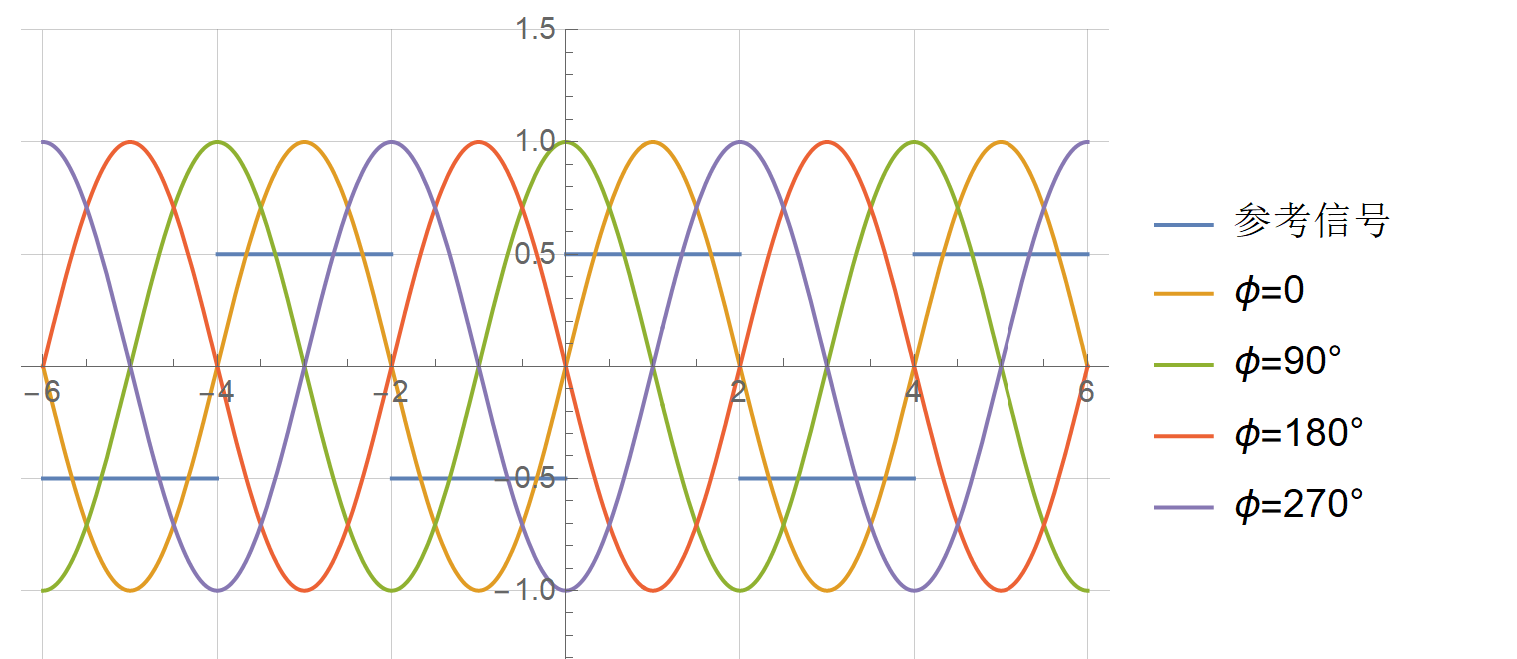
\includegraphics[width=\textwidth]{参考信号相位.png}
    \caption{参考信号与输入信号在不同相位差下的波形图}
    \label{fig:reference-signal-phase}
    \end{figure}

\begin{enumerate}
    \item[1.] 改变参考信号和信号源的相位差时,宽带移相器的输入(正弦波)和输出(方波)波形的相位差也随之进行相同的变化。然而,不同相位差对应的输入和输出波的频率始终是相同的。这一现象与上面得到的参考信号和信号源频率之间的关系一致。
    
    \item[2.] 当将正弦波换为方波或三角波时,输出波仍然为方波,且其相位和频率的变化规律与上述规律相同。
\end{enumerate}

综上, 移相器提供频率可控, 相位可控, 幅度稳定的参考信号.
\subsection{相敏检波器 (PSD) 输出波形和电压测量}

\subsubsection{输入信号、参考信号及PSD的输出波形之间的关系}

实验步骤如下:设置输入信号频率与参考信号频率相同,调整相位差为0°、90°、180°、270°,记录输入信号、参考信号及PSD的输出波形。将交流放大倍数 $K_{AC}=1$,记录波形变化情况。

结果如图所示,显示了宽带移相器的相移量为0°、90°、180°、270°时输入信号、参考信号及PSD输出信号的波形。
\begin{figure}[h]
    \centering
    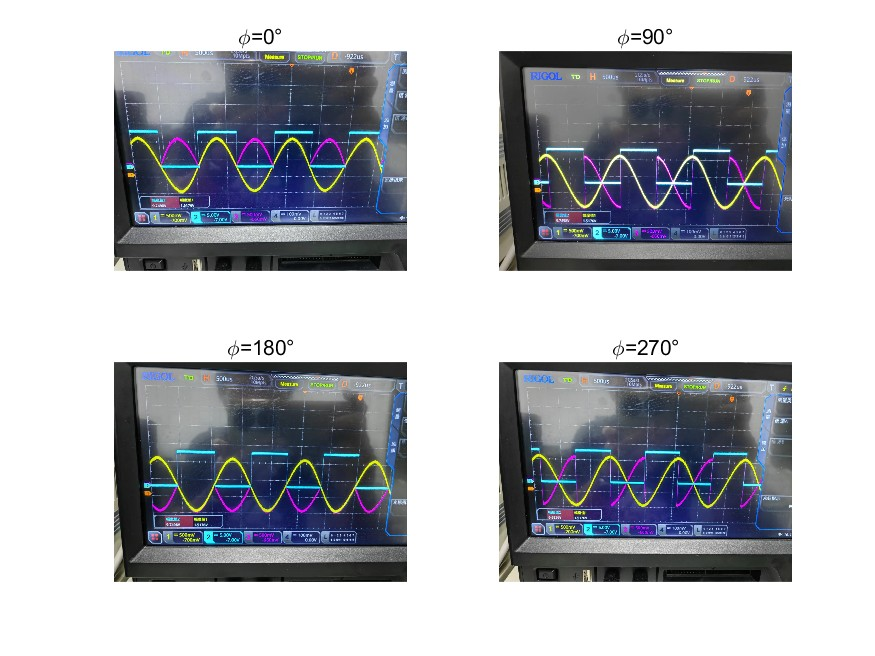
\includegraphics[width=\textwidth]{参考信号相位拼图.jpg}
    \caption{相移量为0°、90°、180°、270°时PSD输出波形}
    \label{fig:reference-signal-phase}
    \end{figure}
其中, 蓝线是参考信号, 黄线是输入信号, 紫线是PSD输出信号. 图中紫线缺失的部分其实是黄线与紫线相重叠, 从中可推知PSD的作用是将输入信号与参考信号相乘。

\subsubsection{探究相关器输出直流电压大小与信号、参考信号之间幅值及相位差 $\phi$ 的关系}

实验设置 $K_{AC}=1$,$K_{DC}=10$,首先控制输入信号幅值为 $V_s=227.7$ mV,探究直流电压大小与相位差 $\phi$ 的关系。

\begin{figure}[H]
    \centering
    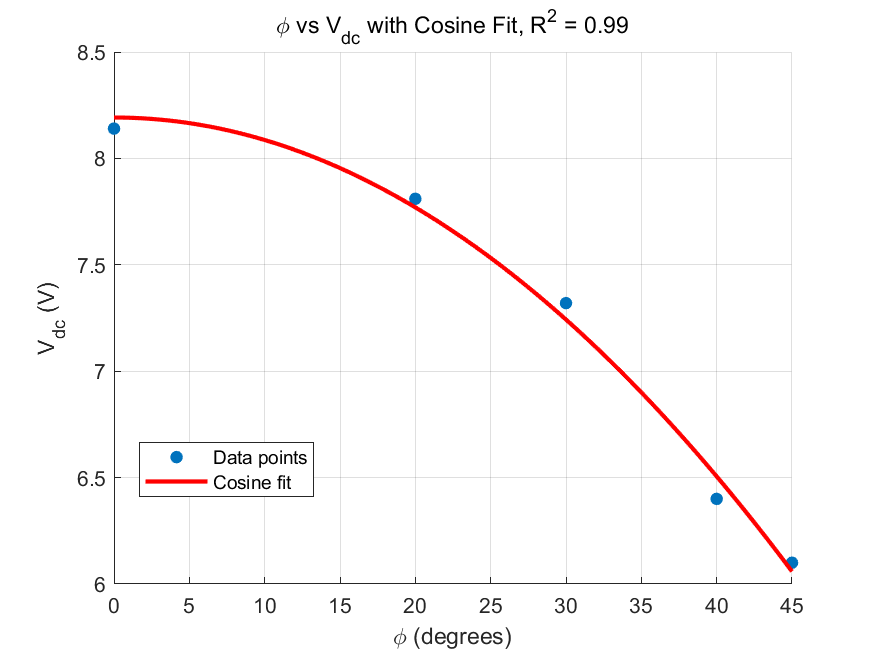
\includegraphics[width=\textwidth]{phi_vs_Vdc_cosine_fit.png}
    \caption{直流电压大小与相位差$\phi$关系}
    \label{fig:phi-vs-Vdc-cosine-fit}
    \end{figure}
可见,PSD输出直流信号与相位差呈余弦关系。相位差$\phi=0$时,直流信号达到最大。

接下来控制$\phi=0°,90°$,探究固定相位差下,直流信号大小与输入信号幅值的关系:
\begin{figure}[H]
    \centering
    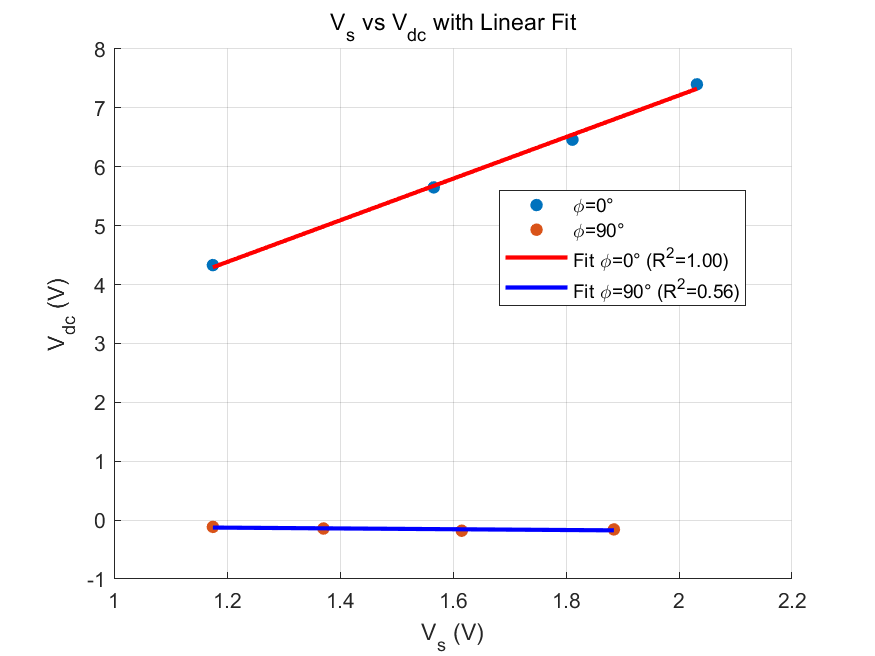
\includegraphics[width=\textwidth]{Vs_vs_Vdc_linear_fit.png}
    \caption{固定相位差$\phi=0°\&90°$下,直流信号大小与输入信号幅值的关系}
    \label{fig:Vs-vs-Vdc-linear-fit}
    \end{figure}
虽然$\phi=90°$时拟合效果不好,但相应的直流信号远远小于0°的情况,说明直流信号与相位差的确符合余弦关系。

\subsubsection{相关器的谐波响应的测量与观察}
将宽带移相器的输入信号接至多功能信号源的“倍频分频输出”,多功能信号源
功能“选择”置“分频”,此时,参考信号的频率为信号频率的 1/n 次倍。
输入信号幅度值为$V_s=227.7$mV时,n与直流信号大小关系如下图所示:
\begin{figure}[H]
    \centering
    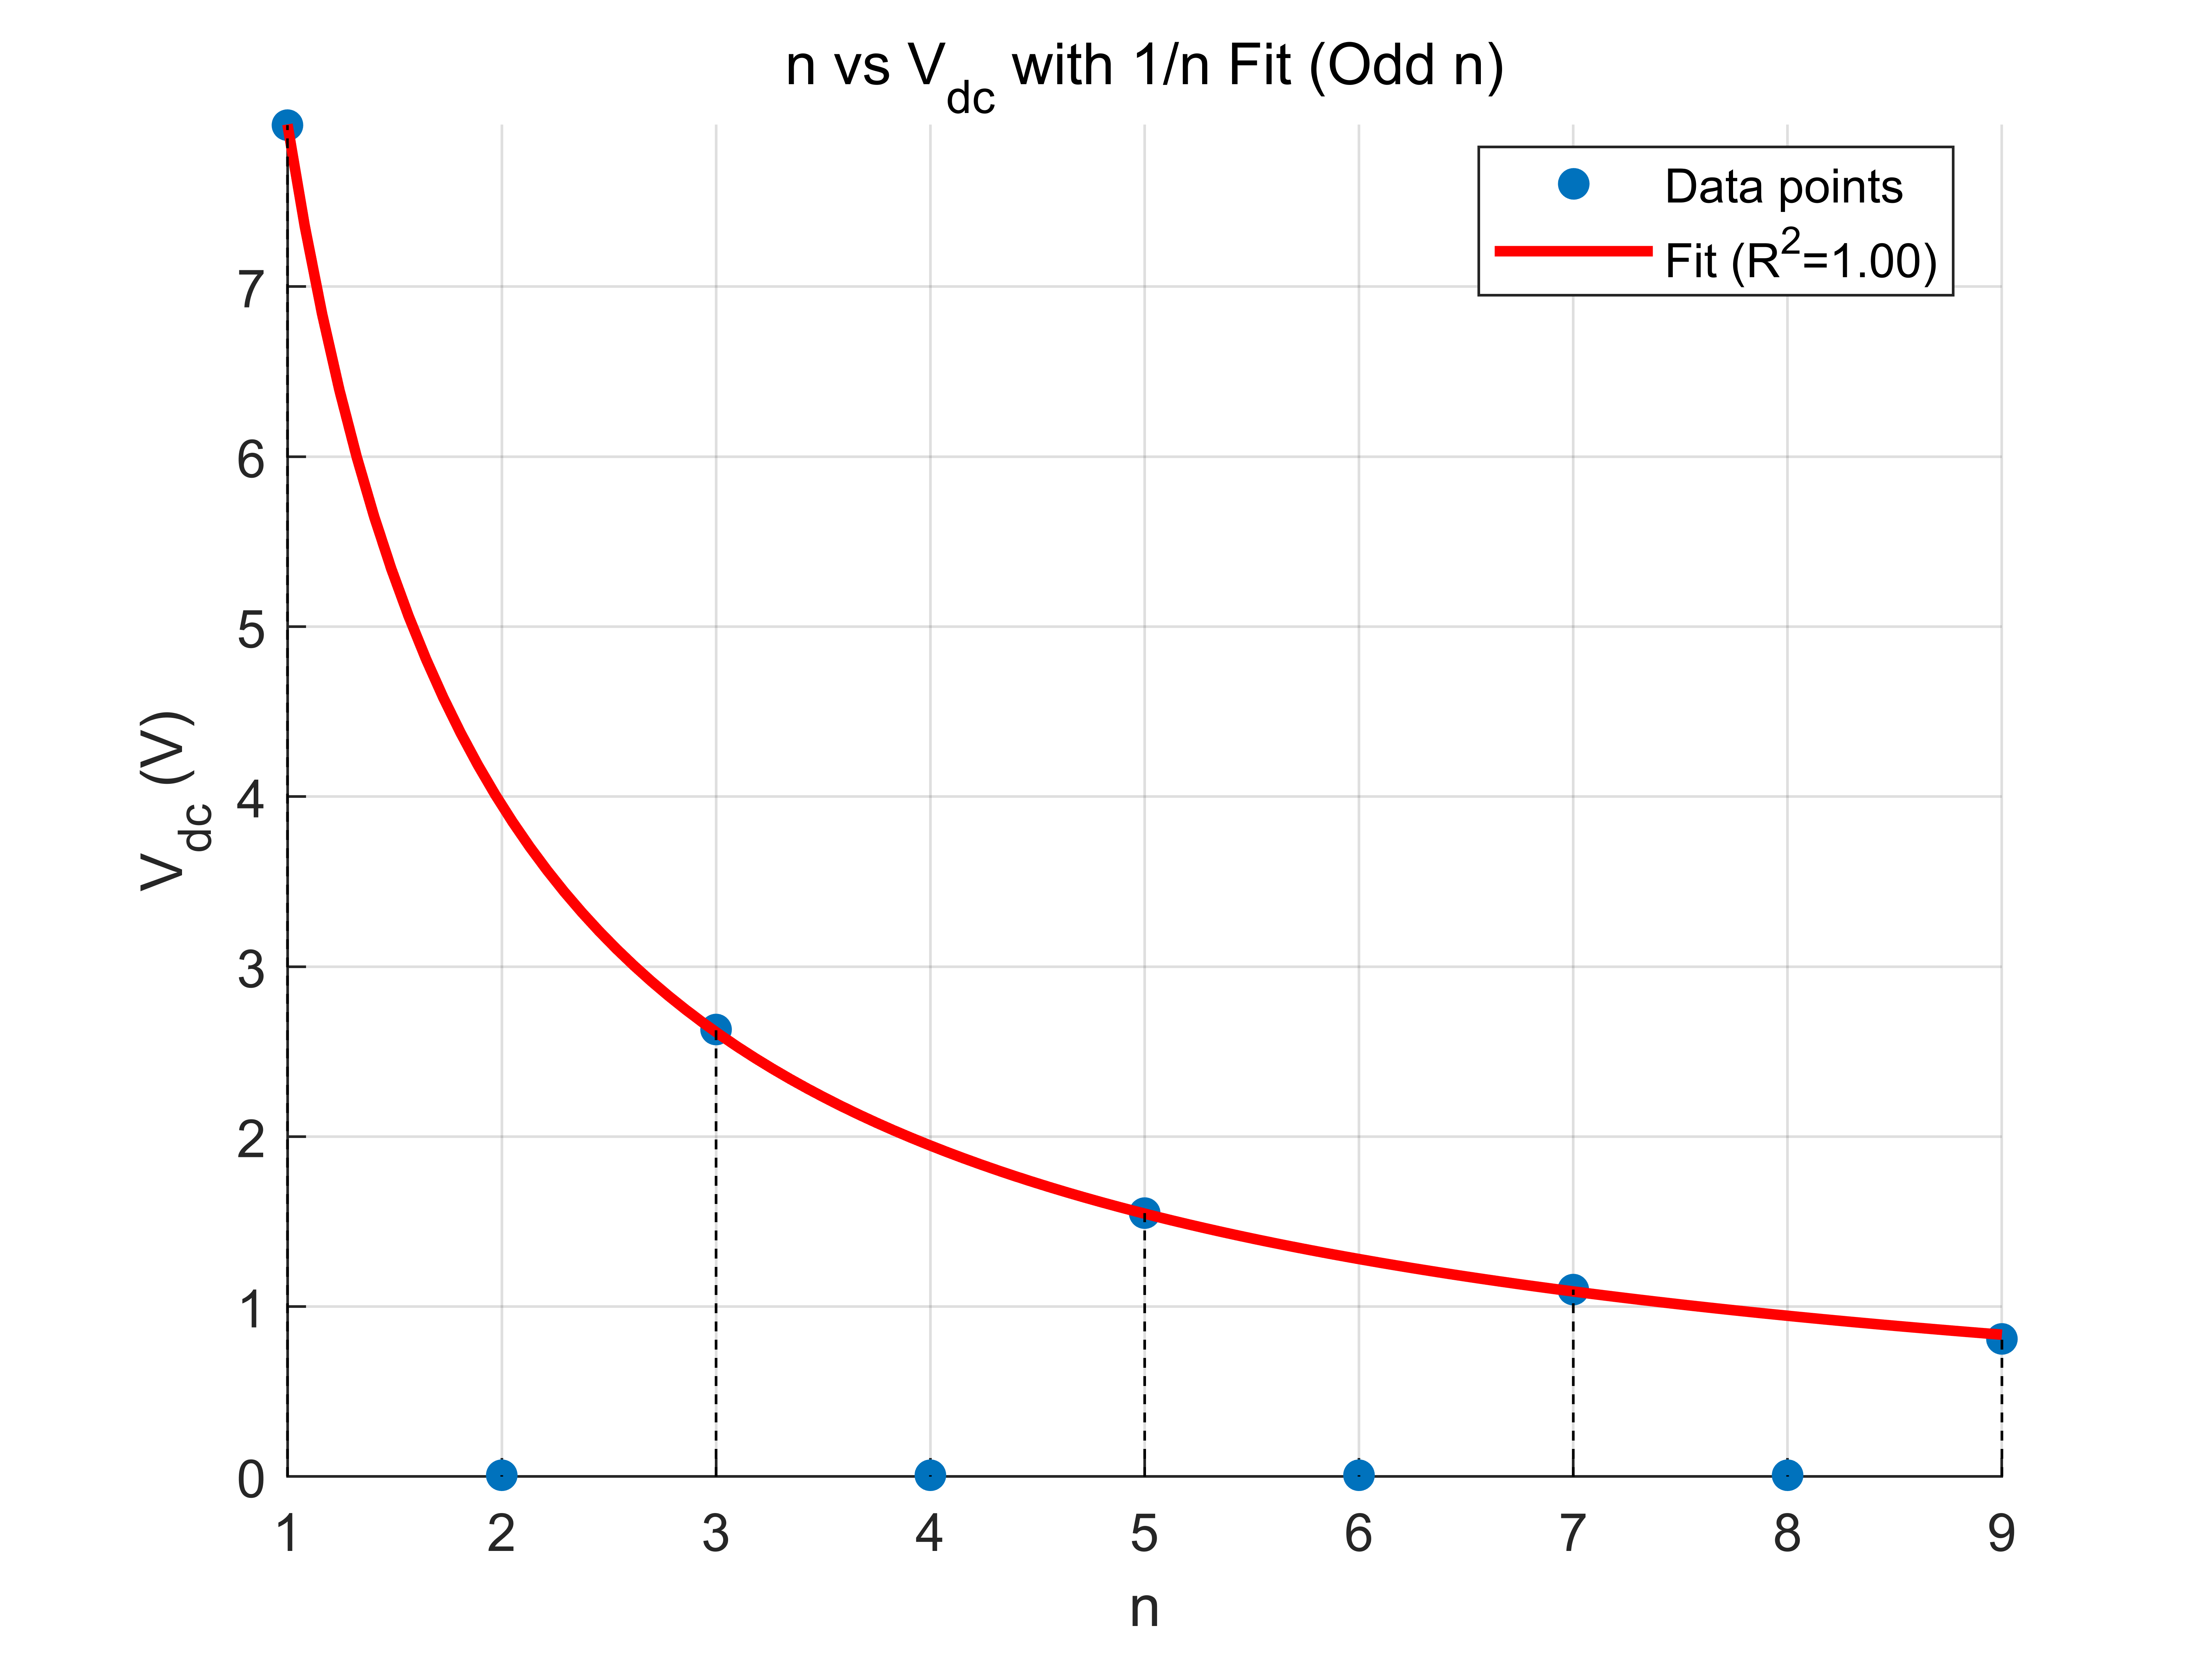
\includegraphics[width=\textwidth]{n_vs_Vdc_fit_odd.png}
    \caption{n与直流信号大小关系}
    \label{fig:n-vs-Vdc-fit-odd}
    \end{figure}
其中发现,只有n为奇数时具有明显的直流信号,且这部分信号按1/n衰减。这表明分频n倍输出且n为奇数时也会产生直流信号,直流信号为正常输出的1/n倍/
\subsubsection{相关器对不相关信号的抑制}
对98mV,f=1006Hz的输入信号,施加幅值为900mV的干扰信号。在无干扰信号时,直流输出的电压$V_dc=1.062V$。改变干扰信号的频率,得到直流电压如下:

\begin{table}[h]
\centering
\begin{tabular}{|c|c|}
\hline
\textbf{频率 (Hz)} & \textbf{直流电压 (V)} \\
\hline
1006 & 0.44-1.627 \\
2012 & 1.063 \\
3018 & 0.995-1.130 \\
4024 & 1.063 \\
5030 & 1.047-1.018 \\
6036 & 1.064 \\
7042 & 1.057-1.072 \\
1500 & 1.064 \\
2500 & 1.064 \\
3500 & 1.064 \\
\hline
\end{tabular}
\caption{干扰信号频率与直流电压数据表}
\label{tab:frequency-voltage-data}
\end{table}
可见当干扰信号频率靠近输入信号的奇次整数倍时,直流电压的范围会出现波动。这是由于干扰信号作为奇次谐波经过乘法器后产生平均值非0的输出信号,由于干扰信号频率与参考信号并不相等,相位差$\phi$一直
在变化,测得的直流信号会围绕1.062V附近进行波动。并且可以观察到,波动的幅度随着n减小。在频率不为奇次整数倍时,不产生直流信号,干扰信号对最终的直流信号的贡献是0,直流信号与无干扰时相同。这表明相关器对奇次谐波的抗干扰能力较差。

\subsubsection{相关器对噪声的抑制及等效噪声带宽}
将均方电压为$\overline{V}=102mV$的白噪声视为干扰信号与$f_s=1.005kHz$与$V_s=57mV$的输入信号混合在一起,此时的信噪比为$r=0.559$. 
经由相关器后,噪声得到抑制,抑制的程度与时间常数T有关:

1. T=1s时,输出信号在4.81-4.91V间波动。将波动用三角函数近似,则波动的方均根也就是噪声为幅值0.1V的$1/2\sqrt{2}$倍。此时信噪比为$r=137$.

2. T=0.1s时,输出信号在4.68-5.06V间波动。信噪比$r=36$.

3. T=10s时,输出信号在4.87-4.88V间波动。基本没有噪声了。
信噪比随时间常数T增大而增大,这是噪声在长周期中被平均的结果。
\section{总结}
本实验使用锁相放大器研究了参考信号通道特性,得到参考信号与信号源频率相等,幅度为固定值,与信号源无关;研究了相敏检波器 PSD 输出波形和电压与信号源和参考信号的关系,得出其在实验误差允许范围内满足公式(4);
研究了相关器对谐波的响应情况,得出当输入信号为参考信号的次谐波时,直流输出信号的幅度最大值与倍数成反比;
研究了干扰信号对PSD直流输出电压的影响,输出电压对干扰信号奇次谐波的抗干扰能力较差。
研究了相关器对噪声的抑制情况,信噪比改善受到输入端信号、输入噪声以及时间常数影响。
\end{document}